\section{Evaluations}
\label{sec:DOICollectionEvaluation}

\subsection{Overview}
We instrumented D{\"o}rk's interactive PivotPaths visualization of multifaceted data~\cite{Dor12}. Figure~\ref{fig:pivotpaths} shows the visualization which links to the popular internet movie database (IMDB). We collected data from $9$ subjects, each using our instrumented visualization for $50$ minutes on a series of structured and unstructured tasks. We used this data to test the validity and effectiveness of our approach in two ways. 

First, we compared the output of the predictive algorithm to human annotations. We found that data collected automatically was on average as similar to human annotations, as human annotations were analogous to each other. We conducted this analysis for all three viewed detection algorithms described in Sections~\ref{sec:AOIBasedViewedObjectDetection} to~\ref{sec:MehthodsIntelligentAlgorithm} and found that the AOI algorithm performs poorly compared to the other two and that the predictive algorithm improves detection accuracy by about $5\%$  (Figure~\ref{fig:quantitative}). 

Second, we showed that our instrumentation method provides relevant information that we can leverage in novel ways. We showed both qualitatively and quantitatively that viewed objects detected automatically were closely correlated to tasks people were asked to do, and that data collected automatically from many users could answer novel questions about how people use visualizations (Figures~\ref{fig:heatmap}~and~\ref{fig:RelevanceDiagram}).    We also demonstrated quantitatively that the viewing-biases our predictive algorithm exploits exist and are significant: our users were much more likely to look at objects that were highlighted and connected to each other (Table~\ref{tab:TransitionFromMovie},~\ref{tab:TransitionFromActor},~\ref{tab:TransitionFromDirector}, and~\ref{tab:TransitionFromGenre}).


\subsection{Instrumenting a Sample Visualization}
\label{sec:InstrumentingVisualization}

\begin{figure}[htb]
  \centering
  \includegraphics[width=\linewidth]{images/PivotPath.eps}
  \caption{PivotPaths visualization of IMDB data. Movies are displayed in the center of the screen, actors at the top, and directors and genres share the bottom space. Actors, directors, and genres associated to movies are connected through curves. Users can highlight objects and their connected neighbors by hovering over them.}
	\label{fig:pivotpaths}
\end{figure}
Our PivotPaths visualization of IMDB data renders movies in the center of the screen, actors on top, and genres and directors at the bottom (Figure~\ref{fig:pivotpaths}). The visualization connects actors, directors, and genres by curves to the associated movies. Moreover, the elements are larger, and their connections more salient, if they associate with multiple movies. Actors, genres, and directors are colored distinctively, which is particularly important for genres and directors since they occupy the same visual space. Such views are created in response to users' searches for specific movies, actors, and directors, and show only data that is most relevant to the search. As shown in Figure~\ref{fig:pivotpaths}, users can hover over visual elements to highlight them and their connections. Users can also click on visual elements to transition the view to one centered on the select element. Finally, users can freely zoom and pan. 

We opted to instrument this visualization for three reasons. First, it is highly interactive and would be significantly difficult to analyze using traditional analyses. Second, it contains visual metaphors, graphic primitives, and interactions typical of a wide range of visualizations. Third, movie data is familiar to a wide variety of users.  

To choose transitions functions $T$ underlying our predictive algorithm, we made simple assumptions about how the visualization is used, an approach also employed by Salvucci~\cite{Sal00}. We assumed that transitions between connected items would occur more often than between unconnected objects. We also assumed that highlighted elements are more likely to be viewed than those that are not. We translated these assumptions into specific weights, as exemplified in Table~\ref{tab:Transition2}. We show in Section~\ref{sec:EvalResults} that these assumptions hold for the instrumented visualization and the subjects that used it in our study. 

\begin{table}[htbp]
\caption{Example transition probabilities in our instrumented visualization (assumed).}
	\centering
		\begin{tabular}{|l|c|}
			\hline
			 \multicolumn{2}{|c|}{Assumed visual and transition weights} \\ \hline
			Movie to unconnected actor & 1\\\hline
			Movie to connected actor & 3\\\hline
			Movie to unconnected genre & 1\\\hline
			Movie to connected genre & 3\\\hline
			Movie to unconnected director & 1\\\hline
			Movie to connected director & 3\\\hline			
		\end{tabular}
	
	\label{tab:Transition2}
\end{table}

Finally, as part of the instrumentation, our system collected screen shots, interactive events (e.g., zooming, panning), raw gaze samples captured at a rate of $120$Hz, and visual elements that users viewed. For each viewed element we recorded the type (i.e., movie, actor, director, genre), its label, its gaze score ($gs$), its prediction score ($ps$), and the aggregated viewing score ($vs$). All recorded data was time stamped.

\subsection{Study Design}
\label{sec:EvalStudyDesign}

\noindent\textbf{Setup: } We used the IMDB visualization described above, and an SMI RED-120Hz connected to a 17'' monitor. Subjects were seated approximately $30''$ away from the display. 

\noindent\textbf{Subjects:} We collected data from $9$ graduate and undergraduate students aged between $20$ and $30$ years. Six subjects were male, and three were female. All were paid $\$10$ for their participation. 

\noindent\textbf{Protocol:} At first, we gave the subjects a description of the study's purpose and protocol. Next, we introduced them to the visualization and asked to perform a few training tasks. This introductory part lasted on average $10$ minutes. The main section of the study followed, involved multiple instances of four types of tasks, and lasted approximately $50$ minutes. 

\noindent\textbf{Tasks:} Subjects completed four types of structured and unstructured tasks. To solve structured tasks, subjects had to consider data that was better defined and less variable than in unstructured tasks. This made it easier for us to test the degree to which object-detection was aligned with the task associated data. On the other hand, data collected in unstructured tasks may be more ecologically valid. We limited the time we allowed subjects to spend on each task for two reasons: to manage the total duration of the study and to make results comparable across users.

\begin{itemize}
\item \textbf{Task1 (structured):} Finding four commonalities between pairs of movies. The tasks were limited at three minutes each, and subjects solved the following four instances of this task: (a) Goodfellas and Raging Bull; (b) Raiders of the Lost Ark and Indiana Jones and the Last Crusade; (c) Invictus and Million Dollar Baby; (d) Inception and The Dark Knight Rises.  
\item \textbf{Task2 (structured):} Ranking collaborations between a director and three actors ($2$ minutes, $4$ instances): (a) Ang Lee; (b) Tim Burton; (c) James Cameron; (d) David Fincher.  
\item \textbf{Task3 (semi-structured):} Given three movies, subjects were asked to recommend a fourth ($5$ minutes, $3$ instances): (a) Catch Me If You Can, E.T. the Extra-Terrestrial, and Captain Phillips; (b) To Kill a Mockingbird, The Big Country, and Ben-Hur; (c) Inglourious Basterds, The Avengers, and Django Unchained.

\item \textbf{Task4 (unstructured):} Given a brief and incomplete description of the ``Brat Pack'', a group of young actors popular in the 80's, subjects were asked to find additional members and movies they acted in. Subjects solved one such task, in approximately $5$ minutes. 
\end{itemize}


\subsection{Results}
\subsubsection{Data Collected Automatically is Similar to that of Human Annotators}
\label{sec:EvalResults}

We tested whether the outputs of the three algorithms described in Sections~\ref{sec:AOIBasedViewedObjectDetection} to~\ref{sec:MehthodsIntelligentAlgorithm} (AOI, probabilistic, and predictive) are comparable to annotation data obtained from human coders who inspected screen-captures with overlaid gaze samples and manually recorded what subjects viewed. We included in our analysis the AOI algorithm version which uses padded AOIs (Section ~\ref{sec:AOIBasedViewedObjectDetection}). As shown in Figure~\ref{fig:quantitative}, we found that the overlap between human annotations and the predictive algorithm's output is similar to the overlap within the set of human annotations and that the predictive algorithm outperforms the others. 

We enlisted the help of five coders and asked them to annotate eye-tracking data corresponding to one task of approximately three minutes, for each of six subjects.  The task was the same for all coders - task 1b. The six subjects were selected randomly and were the same for all five coders. Coders spend approximately one hour per subject completing their annotation. This long duration meant it was unfeasible to code data from more users or more tasks. Four coders completed all six assigned annotation tasks, while one was able to annotate the data of only three subjects. 

Coders used an application that allowed them to browse through screen captures of a users' activity with overlaid gaze coordinates. We asked coders to advance through the videos in $100$ms time-steps, determine what visual objects their assigned subjects were viewing, and record those objects along with the start time and the end time of their viewing. If unsure which of multiple viewed objects, coders were allowed to record all of them.  

We transformed each coder's annotation into temporal vectors with $100$ms resolution. These vectors contained at each position one or several objects that were likely viewed by the subject during each $100$ms time-step. We then created similar representations from our automatically collected data. Finally, we defined a similarity measure between two such vectors as the percentage of temporally aligned cells from each vector that were equal. We defined equality between vector cells as a non-empty intersection between their contents.  

For each algorithm, we computed the similarity of its output for each subject's data to all available human annotations of the same data.  This yielded $4$ coders $\times$ $6$ subjects $+$  $1$ coder $\times$ $3$ subject $=$ $27$ similarities per algorithm. We averaged these similarities and plotted them as the first four bars in Figure~\ref{fig:quantitative}. Then, we compared each coder's annotation of a subject's data to all other available annotations of the same data. Since we had five annotations for three subjects, yielding $3$ subjects $\times$ $10$ annotation pairs $=$ $30$ similarities. Moreover, four annotations for the remaining subjects, yielding $3$ subjects $\times$ $6$ annotation pairs $=$ $18$ similarities. Finally,  we obtained $48$ similarities, which we averaged and plotted as the last bar of Figure~\ref{fig:quantitative}.

The data we collected allowed us to perform this analysis for all three algorithms described in Section~\ref{sec:DOICollectionMethods}, as well as for the padded version of the AOI method. If we only consider gaze scores $gs$ that are equal to one (Section~\ref{sec:AOIBasedViewedObjectDetection}) and no predictive component, we essentially have the output of the AOI algorithm. If we limit the analysis to $gs$ scores alone, without the prediction component described in Section~\ref{sec:MehthodsIntelligentAlgorithm}, we have the output of the probabilistic approach described in Section~\ref{sec:ProbabilisticObjectDetection}.

\begin{figure}[htb]
  \centering
  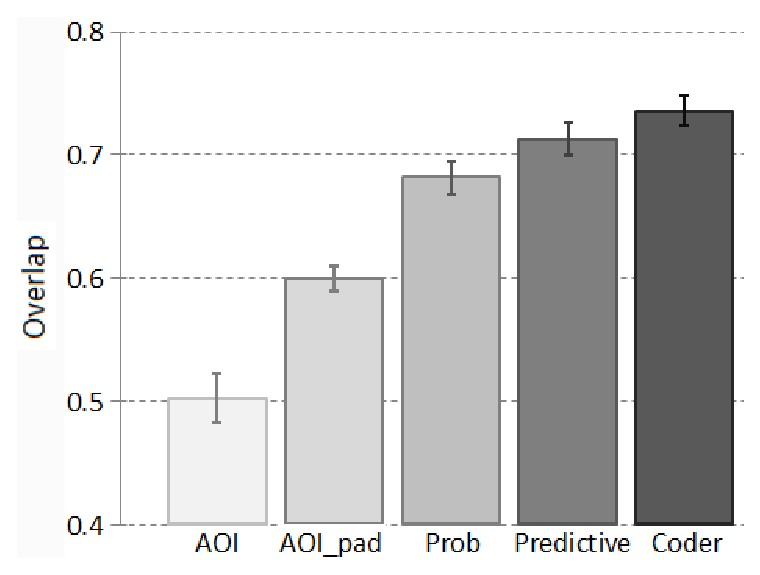
\includegraphics[width=0.6\linewidth]{images/algosComparison.eps}
  \caption{Comparison between automated and manual viewed object detection.
The first four bars show the overlap between the outputs of
the three algorithms described in Section~\ref{sec:DOICollectionMethods} (padded-AOI approach included), and
annotation results of human coders. The last bar shows the overlap
within the set of human annotations. Values correspond to averages
over multiple tasks, multiple subject data sets, and multiple annotators,
and are computed as described in Section~\ref{sec:EvalResults}. Error bars
extend by one standard error. }
	\label{fig:quantitative}
\end{figure}


\subsubsection{Data Collected Automatically is Relevant and Useful}
\label{sec:EvalDataCollected}

We used two analyses to show that data collected automatically is tightly correlated with the tasks that users had to do. We chose this evaluation for two reasons. First, it provides evidence that our instrumentation approach can be used to solve the inverse problem: an observer or analyst who is unfamiliar with a subject's intentions can determine what these are by looking at the subject's visual interest data. 

Second, it demonstrates how the automated collection of eye-tracking data can facilitate novel insights into how we use visualizations. Our approach allowed us to quantify that a users' interest in a visual item present on the screen decays exponentially with a decrease in the items' relevance to a task. It is a well-known fact in visualization community that users follow ``information scent'' when solving tasks visually~\cite{informationscent2003}. Thus, from this fact, we were able to quantify this effect. 
 
\vspace{2mm}\noindent
\textbf{First }, we created heatmap representations from our collected data (Figure~\ref{fig:heatmap}) to illustrate qualitatively the strong connection between the tasks our subjects performed and the data we collected. We listed viewed objects vertically, discretized viewing scores by averaging them over $500ms$ intervals, and arranged them horizontally. Thus, time is shown horizontally, viewed objects vertically, and intensity of heatmap cells indicate the degree to which an object was viewed at a given time. The viewed objects listed vertically were colored based on their type (movie, actor, director, genre) and could be sorted by either first time they were viewed, the amount of viewing activity, or type.

Figure~\ref{fig:heatmap} shows the data collected from a subject performing Task 1b: finding commonalities between two Indiana Jones movies. We notice that elements viewed often are tightly connected to the subjects'  task.   Moreover, we can distinguish a temporal pattern: the movies featured in the task description were viewed throughout the analysis, actors were considered early on, followed by genres, then directors, and ultimately a quick scan of other movies. We observed this pattern for most subjects and thought it was caused by the ordering used in the task's phrasing: we asked subjects to determine actors, genres, and directors that were common between the two movies.   

\begin{figure}[!ht]
  \centering
  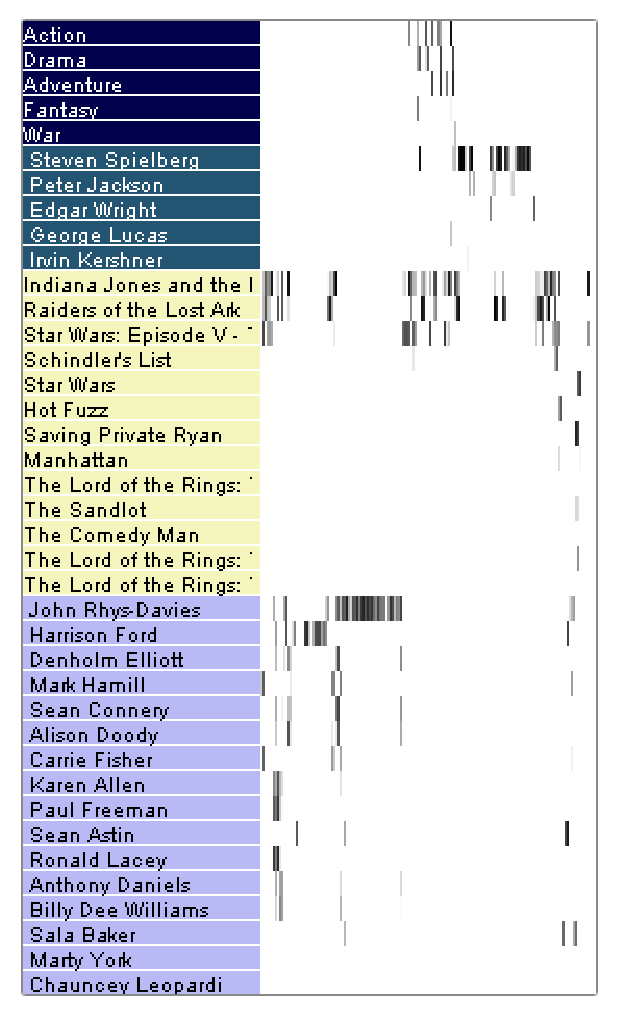
\includegraphics[width=0.75\linewidth]{images/heatmaps.eps}
  \caption{Heatmap views of one subject's activity on Task 1b; time, in 500ms increments, is shown horizontally; viewed objects are viewed vertically; cell darkness indicates viewing intensity (black: high; white: low); viewed items are ordered by category (genre, director, movie, actor). 
}
	\label{fig:heatmap}
\end{figure}

\vspace{2mm}\noindent
\textbf{Second}, we formalized the relevance of each visual item to a particular task and plotted this relevance against the amount of interest that each item attracted (Figure~\ref{fig:RelevanceDiagram}). These plots quantify the degree to which tasks determine users' interest in visual objects and demonstrate that our instrumentation captures relevant data.    

We formalized the relevance of a visual item to a task as $\text{Relevance}~=~1/(1+d)$, where $d$  is the shortest graph distance between that item and items mentioned directly in the task description.  To exemplify, the relevance of Goodfellas and Ranging Bull to task 1a is $1$ as they are the focus of the task, that of Martin Scorsese is $1/2$  because he directed both movies, while that of other movies directed by Scorsese is $1/3$. This definition is not entirely accurate as items might be relevant to a task even though we did not directly mention them in the description.  For instance, items that eventually constitute a user's answer will elicit more attention. 

Figure~\ref{fig:RelevanceDiagram} facilitates several insights. First, even though many items were shown to subjects during their tasks, only very few were viewed for significant periods of time, and many were not viewed at all. Second, the types of user-focused data, correlate with the particularities of each task. For example, Task 3 involved movie recommendations and Figure~\ref{fig:RelevanceDiagram} illustrates that genres and directors were viewed significantly more than in task 4, which involved determining the identity of a group of actors and seemed to drive users' attention towards actors. 

\begin{figure}[!htb]
  \centering
	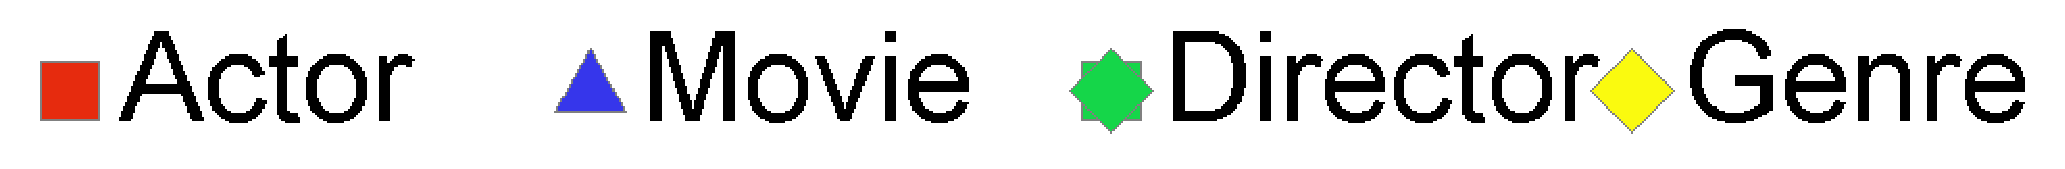
\includegraphics[width=0.45\linewidth]{images/Legends.eps}
  \includegraphics[width=0.6\linewidth]{images/RelevanceDiagramTask1.eps}
	
	\includegraphics[width=0.6\linewidth]{images/RelevanceDiagramTask2.eps}
	
	\includegraphics[width=0.6\linewidth]{images/RelevanceDiagramTask3.eps}
	
	\includegraphics[width=0.6\linewidth]{images/RelevanceDiagramTask4.eps}
	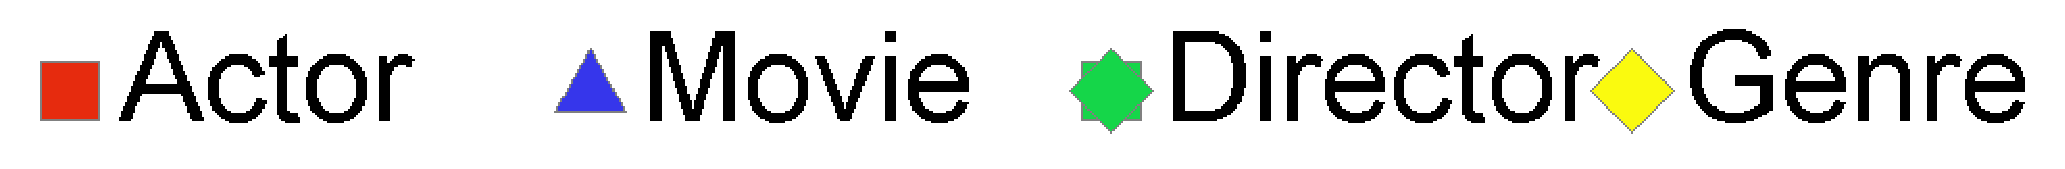
\includegraphics[width=0.45\linewidth]{images/Legends.eps}
	
  \captionof{figure}{Users' interest in data objects, in relation to each objects' relevance to a task, for twelve tasks of four types. Each individual task is plotted in its type's corresponding chart as a subdivision across multiple relevance categories. Relevance was computed as described in Section~\ref{sec:EvalDataCollected}, and plotted for all objects that were visible to subjects during each task. The average interest in objects with the same task relevance are linked by separate polylines for each individual task; errors bars extend from the averages by one standard error.}
	\label{fig:RelevanceDiagram}
\end{figure}



\subsubsection{Viewing Transition Biases Exist and are Significant}
\label{sec:EvalAssumptionAboutViewingTransition}
We performed a quantitative analysis of our subjects' viewing-transition patterns, using the data we collected during our study, and found that the informal assumptions we made in Section~\ref{sec:MehthodsIntelligentAlgorithm} were correct: our users showed strong preferences to view objects that were highlighted or connected to previously viewed objects. The last three columns in Table~\ref{tab:TransitionFromMovie} compare the probability with which our users viewed one object category after another (e.g., viewed a highlighted actor after a movie) as computed from data we collected to a null hypothesis in which users pick at random which items to view next. The quantitative results show for instance that after seeing a movie, our users were four times more likely to look at an actor that was highlighted ($Ratio = 4.081$). Moreover, eleven times more likely to look at an actor that was both highlighted and connected to the previously viewed movie ($Ratio = 11.484$), than if users were viewing items at random.    


To reach these results, we first discarded the prediction component from our data, since it represents exactly the assumption we seek to evaluate. We then counted direct viewing transitions between all types of objects (sources) to all other types of objects (targets) and divided them into categories based on whether targets were highlighted, connected to the sources, or both (Table~\ref{tab:TransitionFromMovie}).  For example, after looking at a movie, our users looked at an actor that was unconnected to that movie and unhighlighted $793$ times, and at an actor that was connect to the movie and highlighted $616$ times. Since in our visualization connections existed only between movies and actors, genres, and directors, transitioning to connected targets was only possible to and from movies.
    

We translated these counts into observed transition probabilities by normalizing them by the total number of transitions from each type of source to each type of category. For example, our users transitioned in total $1784$ times from a movie to an actor, of which $147$ transitions were from a movie to a highlighted actor, yielding an observed transition probability of $147 / 1784 = 0.082$.

However, interpreting these observed probabilities by themselves can be misleading. For example, we observed 793 transitions from a movie to an unconnected actor and just 147 to a connected one. However, This case did not indicate a preference for non-highlighted viewing actors but happened because users had many more opportunities to view unhighlighted actors than they had to view highlighted ones. Intuitively, when a user transitions their gaze from a source to a target, the visualization typically contains many more targets that are not highlighted and are not connected to the source, than those that are. 

Thus, observed transitions should be compared to the default case, which assumes that users treat all visual objects equally. Assume the following simplified case: a movie is connected to two of ten actors shown in a visualization. We observe that of ten transitions from that movie to one of the actors, five were to a connected actor, while five were to unconnected actors. The two observed probabilities, to connected and unconnected actors, would, in this case, be equal at $5/10 = 0.5$. However, if no transitioning preference, the probability of transitioning to any actor would be equal to $0.1$, that of transitioning to a connected actor $0.2$, while that of transitioning to an unconnected actor $0.8$. Thus, our observed transition probability from a movie to a connected actor is $0.5/0.2=2.5$ times higher than the default, unbiased probability, while our observed transition from a movie to an unconnected actor is a fraction ($0.5/0.8=0.625$) of the unbiased one.  

To compute unbiased probabilities, every time we counted a transition from a source to a target, we also counted all target options available to the subject at that point, given the state and structure of the visualization at the time of transition. Reverting to our simplified example, for each of our ten observed transitions we would count two possible transitions to connected actors and eight possible transitions to unconnected actors, ending up with $20$ counts for connected actors, and $80$ counts for unconnected actors. These numbers allow us to compute the two unbiased probabilities as $20/(20+80)$ and $80/(20+80)$.

\begin{table}[htbp]	
\captionof{table}{Transitions from a Movie object to a target object, divided by: (i) type of source and target; (ii) whether the target was highlighted (H); (iii) whether the target was highlighted and connected to the source (HC); (iv) and whether source and target were neither highlighted nor connected. Columns show: (i) the number of direct transitions for the source/target combination; (ii) the observed transition probability from the source to that target; (iii) the (unbiased) probability of transition between source and target if all elements had equal probability to be viewed; (iv) the ratio between observed and unbiased transition probabilities.}
	\centering
		\begin{tabular}{|c|c|c|c|c|c|}
			\hline
			 \multicolumn{2}{ |c| }{Movie to}  &\shortstack{No. of\\transitions} 	&\shortstack{ Observed \\trans.\\prob. }	&\shortstack{	 Unbiased\\trans.\\prob.} & \shortstack{Ratio \\$\frac{\text{Observed}}{\text{Unbiased}}$}\\ \hline
      \multirow{4}{*}{Actor}	&-	&793	&0.445	&0.898	&0.495	\\	\cline{2-6}
															&H	&147	&0.082	&0.02	&4.081	\\	\cline{2-6}
															&C	&228	&0.128	&0.052	&2.473	\\	\cline{2-6}
															&CH	&616	&0.345	&0.03	&11.484	\\	\hline
				\multirow{2}{*}{Movie}	&-	&5727	&0.761	&0.899	&0.846	\\	\cline{2-6}
																&H	&1798	&0.239	&0.101	&2.376	\\	\hline
				\multirow{4}{*}{Director}	&-	&304	&0.537	&0.887	&0.606	\\	\cline{2-6}
																	&H	&37	&0.065	&0.021	&3.088	\\	\cline{2-6}
																	&C	&51	&0.09	&0.055	&1.647	\\	\cline{2-6}
																	&CH	&174	&0.307	&0.038	&8.176	\\	\hline
				\multirow{4}{*}{Genre}	&-	&193	&0.33	&0.792	&0.417	\\	\cline{2-6}
																&H	&40	&0.068	&0.033	&2.045	\\	\cline{2-6}
																&C	&69	&0.118	&0.102	&1.159	\\	\cline{2-6}
																&CH	&282	&0.483	&0.072	&6.693	\\	
				\hline
		\end{tabular}
		
	\label{tab:TransitionFromMovie}
\end{table}

\begin{table}[htbp]	
\captionof{table}{Transitions from Actor objects. }
	\centering
	\begin{tabular}{|c|c|c|c|c|c|}
			\hline
			 \multicolumn{2}{ |c| }{Actor to}    &\shortstack{No. of\\transitions} 	&\shortstack{ Observed \\trans.\\prob. }	&\shortstack{	 Unbiased\\trans.\\prob.} & \shortstack{Ratio \\$\frac{\text{Observed}}{\text{Unbiased}}$}\\ \hline
						 \multirow{2}{*}{Actor}	&-	&4711	&0.685	&0.962	&0.713	\\	\cline{2-6}
																		&H	&2164	&0.315	&0.038	&8.207	\\	\hline
							\multirow{4}{*}{Movie}	&-	&839	&0.469	&0.82	&0.572	\\	\cline{2-6}
																			&H	&213	&0.119	&0.058	&2.046	\\	\cline{2-6}
																			&C	&386	&0.216	&0.076	&2.843	\\	\cline{2-6}
																			&CH	&352	&0.197	&0.046	&4.284	\\	\hline
							\multirow{2}{*}{Director}	&-	&68	&0.701	&0.959	&0.731	\\	\cline{2-6}
																				&H	&29	&0.299	&0.041	&7.271	\\	\hline
							\multirow{2}{*}{Genre}	&-	&43	&0.524	&0.931	&0.563	\\	\cline{2-6}
																			&H	&39	&0.476	&0.069	&6.918	\\	
				\hline
		\end{tabular}
		
	\label{tab:TransitionFromActor}
\end{table}

\begin{table}[htbp]	
\captionof{table}{Transitions from Director objects}
	\centering
\begin{tabular}{|c|c|c|c|c|c|}
			\hline
			 \multicolumn{2}{ |c| }{Director to}    &\shortstack{No. of\\transitions} 	&\shortstack{ Observed \\trans.\\prob. }	&\shortstack{	 Unbiased\\trans.\\prob.} & \shortstack{Ratio \\$\frac{\text{Observed}}{\text{Unbiased}}$}\\ \hline
       \multirow{2}{*}{Actor}	&-	&71	&0.747	&0.958	&0.78	\\	\cline{2-6}
															&H	&24	&0.253	&0.042	&5.964	\\	\hline
			\multirow{4}{*}{Movie}	&-	&271	&0.494	&0.792	&0.623	\\	\cline{2-6}
															&H	&55	&0.1	&0.04	&2.478	\\	\cline{2-6}
															&C	&130	&0.237	&0.108	&2.198	\\	\cline{2-6}
															&CH	&93	&0.169	&0.06	&2.841	\\	\hline
			\multirow{2}{*}{Director}	&-	&384	&0.706	&0.93	&0.759	\\	\cline{2-6}
																&H	&160	&0.294	&0.07	&4.216	\\	\hline
			\multirow{2}{*}{Genre}	&-	&256	&0.522	&0.899	&0.581	\\	\cline{2-6}
															&H	&234	&0.478	&0.101	&4.708	\\	
				\hline
		\end{tabular}
		
	\label{tab:TransitionFromDirector}
\end{table}

\begin{table}[htbp]	
\captionof{table}{Transitions from Genre objects}
	\centering
	\begin{tabular}{|c|c|c|c|c|c|}
			\hline
			 \multicolumn{2}{ |c| }{Genre to}   &\shortstack{No. of\\transitions} 	&\shortstack{ Observed \\trans.\\prob. }	&\shortstack{	 Unbiased\\trans.\\prob.} & \shortstack{Ratio \\$\frac{\text{Observed}}{\text{Unbiased}}$}\\ \hline
			 \multirow{2}{*}{Actor}	&-	&61	&0.656	&0.9791	&0.67	\\	\cline{2-6}
															&H	&32	&0.344	&0.021	&16.47	\\	\hline
				\multirow{4}{*}{Movie}	&-	&229	&0.118	&0.261	&0.453	\\	\cline{2-6}
																&H	&46	&0.024	&0.008	&3.001	\\	\cline{2-6}
																&C	&172	&0.089	&0.093	&0.956	\\	\cline{2-6}
																&CH	&138	&0.071	&0.013	&5.288	\\	\hline
				\multirow{2}{*}{Director}	&-	&282	&0.591	&0.973	&0.608	\\	\cline{2-6}
																	&H	&195	&0.409	&0.027	&15.174	\\	\hline
				\multirow{2}{*}{Genre}	&-	&348	&0.398	&0.943	&0.422	\\	\cline{2-6}
																&H	&526	&0.602	&0.057	&10.627	\\	
				\hline
		\end{tabular}		
		
	\label{tab:TransitionFromGenre}
\end{table}
%\begin{table}[htbp]	
	%\centering
		%\begin{tabular}{|c|c|c|c|c|c|}
			%\hline
			 %\multicolumn{2}{ |c| }{Movie to}  &\shortstack{No. of\\transitions} 	&\shortstack{ Observed \\trans.\\prob. }	&\shortstack{	 Unbiased\\trans.\\prob.} & \shortstack{Ratio \\$\frac{\text{Observed}}{\text{Unbiased}}$}\\ \hline
      %\multirow{4}{*}{Actor}	&-	&793	&0.445	&0.898	&0.495	\\	\cline{2-6}
															%&H	&147	&0.082	&0.02	&4.081	\\	\cline{2-6}
															%&C	&228	&0.128	&0.052	&2.473	\\	\cline{2-6}
															%&CH	&616	&0.345	&0.03	&11.484	\\	\hline
				%\multirow{2}{*}{Movie}	&-	&5727	&0.761	&0.899	&0.846	\\	\cline{2-6}
																%&H	&1798	&0.239	&0.101	&2.376	\\	\hline
				%\multirow{4}{*}{Director}	&-	&304	&0.537	&0.887	&0.606	\\	\cline{2-6}
																	%&H	&37	&0.065	&0.021	&3.088	\\	\cline{2-6}
																	%&C	&51	&0.09	&0.055	&1.647	\\	\cline{2-6}
																	%&CH	&174	&0.307	&0.038	&8.176	\\	\hline
				%\multirow{4}{*}{Genre}	&-	&193	&0.33	&0.792	&0.417	\\	\cline{2-6}
																%&H	&40	&0.068	&0.033	&2.045	\\	\cline{2-6}
																%&C	&69	&0.118	&0.102	&1.159	\\	\cline{2-6}
																%&CH	&282	&0.483	&0.072	&6.693	\\	
				%\hline
		%\end{tabular}		
		%\caption*{(a)Transitions from Movies}
		%\smallskip
		%
		%\begin{tabular}{|c|c|c|c|c|c|}
			%\hline
			 %\multicolumn{2}{ |c| }{Actor to}    &\shortstack{No. of\\transitions} 	&\shortstack{ Observed \\trans.\\prob. }	&\shortstack{	 Unbiased\\trans.\\prob.} & \shortstack{Ratio \\$\frac{\text{Observed}}{\text{Unbiased}}$}\\ \hline
						 %\multirow{2}{*}{Actor}	&-	&4711	&0.685	&0.962	&0.713	\\	\cline{2-6}
																		%&H	&2164	&0.315	&0.038	&8.207	\\	\hline
							%\multirow{4}{*}{Movie}	&-	&839	&0.469	&0.82	&0.572	\\	\cline{2-6}
																			%&H	&213	&0.119	&0.058	&2.046	\\	\cline{2-6}
																			%&C	&386	&0.216	&0.076	&2.843	\\	\cline{2-6}
																			%&CH	&352	&0.197	&0.046	&4.284	\\	\hline
							%\multirow{2}{*}{Director}	&-	&68	&0.701	&0.959	&0.731	\\	\cline{2-6}
																				%&H	&29	&0.299	&0.041	&7.271	\\	\hline
							%\multirow{2}{*}{Genre}	&-	&43	&0.524	&0.931	&0.563	\\	\cline{2-6}
																			%&H	&39	&0.476	&0.069	&6.918	\\	
				%\hline
		%\end{tabular}
	%\caption*{(b)Transitions from Actors}
	%\smallskip
	%
	%\begin{tabular}{|c|c|c|c|c|c|}
			%\hline
			 %\multicolumn{2}{ |c| }{Director to}    &\shortstack{No. of\\transitions} 	&\shortstack{ Observed \\trans.\\prob. }	&\shortstack{	 Unbiased\\trans.\\prob.} & \shortstack{Ratio \\$\frac{\text{Observed}}{\text{Unbiased}}$}\\ \hline
       %\multirow{2}{*}{Actor}	&-	&71	&0.747	&0.958	&0.78	\\	\cline{2-6}
															%&H	&24	&0.253	&0.042	&5.964	\\	\hline
			%\multirow{4}{*}{Movie}	&-	&271	&0.494	&0.792	&0.623	\\	\cline{2-6}
															%&H	&55	&0.1	&0.04	&2.478	\\	\cline{2-6}
															%&C	&130	&0.237	&0.108	&2.198	\\	\cline{2-6}
															%&CH	&93	&0.169	&0.06	&2.841	\\	\hline
			%\multirow{2}{*}{Director}	&-	&384	&0.706	&0.93	&0.759	\\	\cline{2-6}
																%&H	&160	&0.294	&0.07	&4.216	\\	\hline
			%\multirow{2}{*}{Genre}	&-	&256	&0.522	&0.899	&0.581	\\	\cline{2-6}
															%&H	&234	&0.478	&0.101	&4.708	\\	
				%\hline
		%\end{tabular}
		%\caption*{(c)Transitions from Director}
		%\smallskip
		%
		%\begin{tabular}{|c|c|c|c|c|c|}
			%\hline
			 %\multicolumn{2}{ |c| }{Genre to}   &\shortstack{No. of\\transitions} 	&\shortstack{ Observed \\trans.\\prob. }	&\shortstack{	 Unbiased\\trans.\\prob.} & \shortstack{Ratio \\$\frac{\text{Observed}}{\text{Unbiased}}$}\\ \hline
			 %\multirow{2}{*}{Actor}	&-	&61	&0.656	&0.9791	&0.67	\\	\cline{2-6}
															%&H	&32	&0.344	&0.021	&16.47	\\	\hline
				%\multirow{4}{*}{Movie}	&-	&229	&0.118	&0.261	&0.453	\\	\cline{2-6}
																%&H	&46	&0.024	&0.008	&3.001	\\	\cline{2-6}
																%&C	&172	&0.089	&0.093	&0.956	\\	\cline{2-6}
																%&CH	&138	&0.071	&0.013	&5.288	\\	\hline
				%\multirow{2}{*}{Director}	&-	&282	&0.591	&0.973	&0.608	\\	\cline{2-6}
																	%&H	&195	&0.409	&0.027	&15.174	\\	\hline
				%\multirow{2}{*}{Genre}	&-	&348	&0.398	&0.943	&0.422	\\	\cline{2-6}
																%&H	&526	&0.602	&0.057	&10.627	\\	
				%\hline
		%\end{tabular}
		%\caption*{(d)Transitions from Genres}\smallskip
	%\captionof{table}{Transitions from a source object to a target object, divided by: (i) type of source and target; (ii) whether the target was highlighted (H); (iii) whether the target was highlighted and connected to the source (HC); (iv) and whether source and target were neither highlighted nor connected. Columns show: (i) the number of direct transitions for the source/target combination; (ii) the observed transition probability from the source to that target; (iii) the (unbiased) probability of transition between source and target if all elements had equal probability to be viewed; (iv) the ratio between observed and unbiased transition probabilities.}
	%\label{tab:TransitionFromMovie}
%\end{table}